\documentclass[11pt,a4paper]{article}

%==============================================================================%

\usepackage{a4wide}
\usepackage{amsmath,amssymb}
\usepackage[utf8]{inputenc}
\usepackage{float}
\usepackage{graphicx}
\usepackage{listings}
\usepackage{multicol}

%==============================================================================%

\newcommand{\assignmentnumber}{1}
\newcommand{\modulus}[1]{\lvert#1\rvert}
\newcommand{\conjugate}[1]{\bar{#1}}
\newcommand{\degree}{^{\circ}}

\DeclareMathOperator{\re}{Re}
\DeclareMathOperator{\im}{Im}

\renewcommand\thesection{\assignmentnumber.\arabic{section}}
\renewcommand\thesubsection{\alph{subsection})}

%==============================================================================%

\title{MatIntro Lynopgave \assignmentnumber}
\author
{
    Casper B. Hansen\\
    University of Copenhagen\\
    {\tt fvx507@alumni.ku.dk}
}
\date{\today}

%==============================================================================%

\begin{document}

% \maketitle

\section
{
    \mdseries Betragt funktionerne $f_1 = \frac{x^2 - 7}{x + \sqrt{7}}$ og
    $f_2 = \frac{x^2 - 7}{x + 2.645751311}$.
    Lav et Maple-plot af graferne for de to funktioner med $x$ i intervallet
    $[-2.6458,-2.6457]$. Forklar, hvad du ser.
}
Som det fremgår af graferne nedenfor, er grafen for $f_1$ kontinuert,
hvorimod approksimeringen af $\sqrt{7}$ giver et brud i grafen for $f_2$,
hvilket gør at grafen ikke er kontinuerlig. Dette sker i $x = -2.645751311$,
da nævneren for brøken da vil være lig $0$.

\begin{multicols}{2}

    \begin{figure}[H]
        \center
        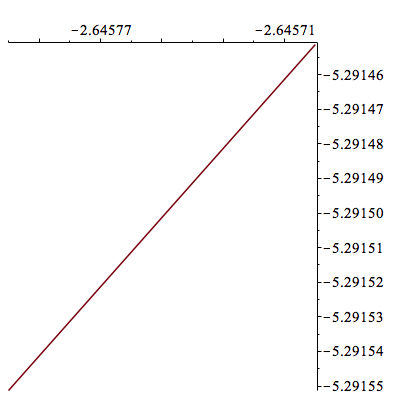
\includegraphics[scale=0.5]{figures/f1.png}
        \caption{Graf for funktionen $f_1$}
    \end{figure}

    \vfill\columnbreak

    \begin{figure}[H]
        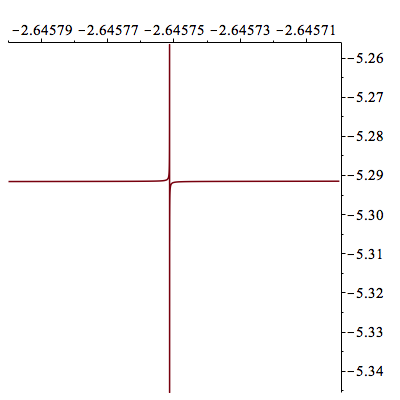
\includegraphics[scale=0.5]{figures/f2.png}
        \caption{Graf for funktionen $f_2$}
    \end{figure}

\end{multicols}

\section{\mdseries
    Lad $z = 3 + 4i$ og $w = 2 + i$
}

\subsection{\mdseries
    Bestem hvert af tallene $z - 2w$, $iz + w$, $zw$, $\frac{z}{w}$ og $w^2$
}

\begin{multicols}{3}
    
    \begin{align*}
        z - 2w &= (3 + 4i) - 2(2 + i) \\
               &= (3 + 4i) - (4 + 2i) \\
               &= 3 - 4 + 4i - 2i \\
               &= -1 + 2i
    \end{align*}

    \begin{align*}
        iz + w &= i(3 + 4i) + (2 + i) \\
               &= 3i + 4i^2 + (2 + i) \\
               &= (-4 + 3i) + (2 + i) \\
               &= -2 + 4i
    \end{align*}

    \vfill\columnbreak

    \begin{align*}
        zw &= (3 + 4i)(2 + i) \\
           &= 6 + 3i + 4i^2 + 8i \\
           &= 2 + 11i
    \end{align*}

    \begin{align*}
        \frac{z}{w} = \frac{z\conjugate{w}}{w\conjugate{w}}
                   &= \frac{(3 + 4i)(2 - i)}{(2 + i)(2 - i)} \\
                   &= \frac{6 - 3i + 8i + 4i(-i)}{4 - 2i + 2i + i(-i)} \\
                   &= \frac{10 + 5i}{5} \\
                   &= 2 + i
    \end{align*}
    
    \vfill\columnbreak

    \begin{align*}
        w^2 &= (2 + i)(2 + i) \\
            &= 2^2 + i^2 + 2 \cdot 2 i \\
            &= 4 - 1 + 4i \\
            &= 3 + 4i
    \end{align*}

    \vfill

\end{multicols}

\subsection{\mdseries
    Bestem endvidere modulus og argument for $w$.
}
\begin{align*}
    \modulus{w} = \sqrt{\re(w)^2 + \im(w)^2}
                = \sqrt{2^2 + 1^2}
                = \sqrt{5}
    \qquad
    w_\theta = \tan^{-1}\left(\frac{\im(w)}{\re(w)}\right)
             = \tan^{-1}\left(\frac{1}{2}\right)
             \approx 26.6\degree
\end{align*}

\section{\mdseries
    Lad $w = \frac
        {
        \left(
            \frac{3}{4} + \frac{1}{2}i
        \right)
        \left(
             \frac{1}{4} - \frac{3}{2}i
        \right)
        }
        {
        \left(
            -\frac{1}{4} + \frac{1}{2}i
        \right)
        }$
}

\subsection{\mdseries Udregn modulus og argument af det komplekse tal $w$ og
    indtegn det i den komplekse plan}
Først og fremmest simplicerer vi $z$ og får da, at
\begin{align*}
    w = -\frac{8}{5} + \frac{1}{5}i
\end{align*}

Dernæst finder vi modulus
\begin{align*}
    \modulus{w} &=
    \sqrt{
        \left(-\frac{8}{5}\right)^2 +
        \left(-\frac{1}{5}\right)^2}
    = \frac{1}{5}\sqrt{65}
\end{align*}

Og argumentet
\begin{align*}
    w_\theta &= \tan^{-1}\left( \frac{ -\frac{1}{5} }{ -\frac{8}{5} } \right)
              = \tan^{-1}\left( -\frac{1}{8} \right)
              = \tan^{-1}\left( \frac{1}{8} \right) - \pi
\end{align*}

\subsection{\mdseries Lad $z = \frac{3}{4} + \frac{1}{2}i$. Indtegn tallene
$z^{-8}$, $z^{-7}$, \dots, $z^{-1}$, $z^0$, $z$, $z^2$, \dots, $z^8$ i den
komplekse plan og forklar resultatet.}

\begin{multicols}{2}

Med udgangspunkt i $z^x$ ser vi for $\{x \in Z | x > 0\}$ bevæger vi
os $z_\theta$ modsat urets retning om origo. Modsat, for $\{x \in Z | x \leq
0\}$ bevæger vi os med urets retning om origo. Det fremgår også, at $z^0$ er
et reelt tal, da $z_\theta = 0$.

\vfill\columnbreak

\begin{figure}[H]
    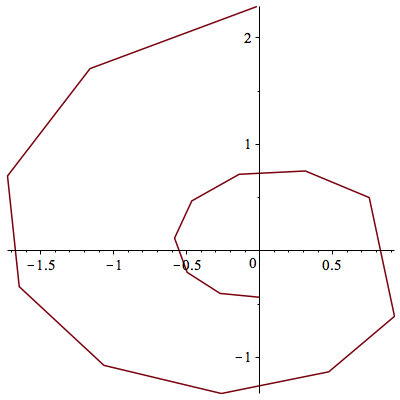
\includegraphics[scale=0.5]{figures/fib.png}
    \caption{Plot i den komplekse plan over $z^x$, hvor $x \in \{-8,\dots,8\}$}
\end{figure}

\end{multicols}

\end{document}
